\documentclass[]{beamer}

% This file is a solution template for:

% - Giving a talk on some subject.
% - The talk is between 15min and 45min long.
% - Style is ornate.



% Copyright 2004 by Till Tantau <tantau@users.sourceforge.net>.
%
% In principle, this file can be redistributed and/or modified under
% the terms of the GNU Public License, version 2.
%
% However, this file is supposed to be a template to be modified
% for your own needs. For this reason, if you use this file as a
% template and not specifically distribute it as part of a another
% package/program, I grant the extra permission to freely copy and
% modify this file as you see fit and even to delete this copyright
% notice.


\mode<presentation>
{
  \usetheme{Montpellier}
  \usecolortheme{dolphin}
  \setbeamercovered{transparent}
}


\usepackage[english]{babel}
\usepackage{alltt}
\usepackage[latin1]{inputenc}
\usepackage{times}
\usepackage[T1]{fontenc}


\title[]{Giant Cow Games}
\subtitle{Darkmatter}
\author[]{J. Greenaway \and C. Horrell \and Y. Wang \and J. Via}
\date[]{23 March 2011}


% If you have a file called "university-logo-filename.xxx", where xxx
% is a graphic format that can be processed by latex or pdflatex,
% resp., then you can add a logo as follows:

\pgfdeclareimage[height=0.5cm]{logo}{img/logo.png}
\logo{\pgfuseimage{logo}}


% Delete this, if you do not want the table of contents to pop up at
% the beginning of each subsection:
\AtBeginSubsection[]
{
  \begin{frame}<beamer>{Outline}
    \tableofcontents[currentsection,currentsubsection]
  \end{frame}
}


% If you wish to uncover everything in a step-wise fashion, uncomment
% the following command:

% \beamerdefaultoverlayspecification{<+->}


\begin{document}

\begin{frame}
  \titlepage
\end{frame}

\begin{frame}{Outline}
  \small\tableofcontents
\end{frame}



\section{Introduction}

\subsection{Inspiration}
%%
%% Talk about our inspiration for the game.
%%
\begin{frame}{Osmos}
  \begin{figure}
    % Source:
    % http://blog.brettalton.com/wp-content/uploads/osmos-running-on-linux.png
    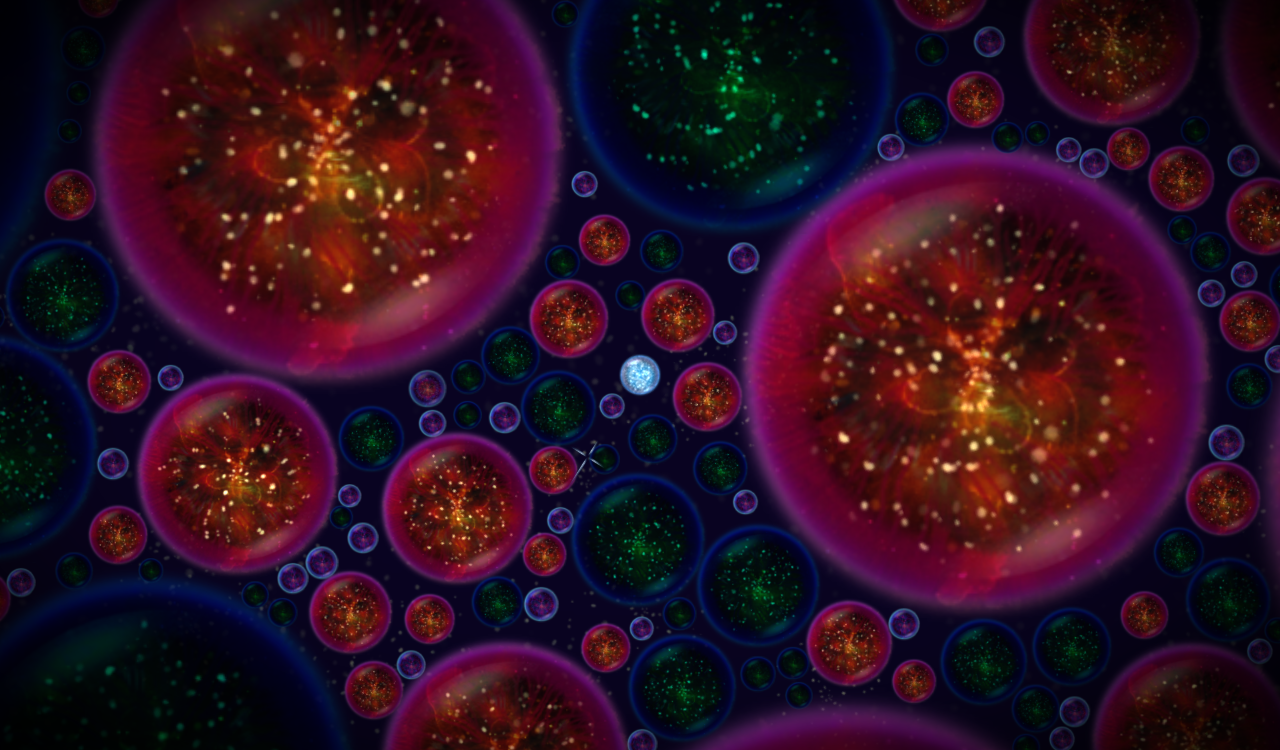
\includegraphics[width=0.6\textwidth]{img/osmos.png}
  \end{figure}
  \begin{block}{}
    A beautiful puzzle game created by Hemisphere games.
  \end{block}
\end{frame}


\subsection{Darkmatter}
\begin{frame}{Early Prototype}
  %% Notes:
  %% - talk about how the game has a simple core and can be expanded
  %% - making the game mulitplayer changes the dynamic
  \begin{figure}
    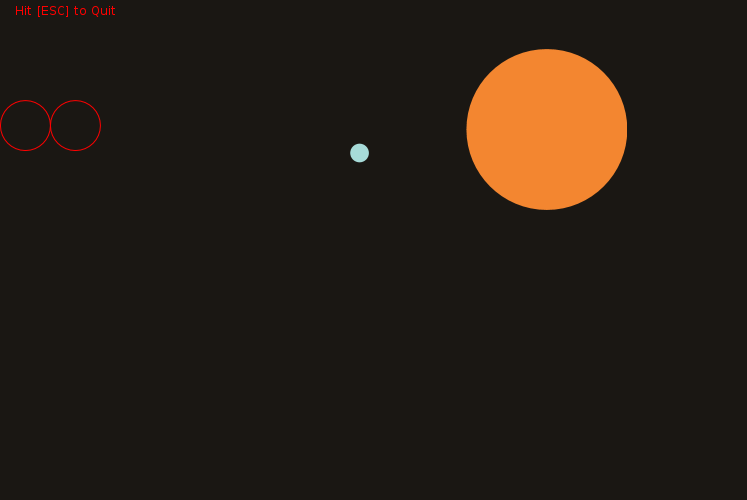
\includegraphics[width=0.8\textwidth]{img/prototype.png}
  \end{figure}
\end{frame}

\begin{frame}{Final Version}
  %% Notes:
  %% -
  %%
  \begin{figure}
    
\includegraphics[width=0.8\textwidth]{img/final.png}
  \end{figure}
\end{frame}

\begin{frame}{The Future}
  %% Notes:
  %% - adding defensive powerups
  %% - co-op mode instead of against
  %% - completing sub-tasks
  \begin{figure}
    
\includegraphics[width=0.6\textwidth]{img/future.png}
  \end{figure}
  \begin{block}{Enhancements}
    \begin{itemize}
    \item Defensive power-ups
    \item Co-op mode
    \item Completing missions
    \end{itemize}
  \end{block}
\end{frame}



\section{Game Time}
%%
%% Run the game demo but keep it short and straight to the point.
%%
\begin{frame}{}
  And here we go...
\end{frame}



\section{Extreme Programming}
%%
%% Our reasons for using XP.
%%
\begin{frame}{Why XP?}
  \begin{block}{}
    \begin{itemize}
    \item Release early \& release often \\
      We built a small core and added functionality feature by
      feature.
    \item Collective code ownership \\
      We are all responsible for fixing bugs in any file.
    \item Planning game \\
      We all had a sense of how much effort a feature required.
    \end{itemize}
  \end{block}
\end{frame}

%%
%% Talk about how we deviated from XP.
%%
\begin{frame}{But we weren't perfect}
  \begin{itemize}
  \item \emph{Not as many release as we aimed for.} \\
    Hard to remember to create tags whenever a feature milestone was
    reached.
  \item We coded our \emph{unit tests after our features}. \\
    New domain = exploratory coding.
  \item \emph{No overtime.} \\
    We can't push back client deadlines.
  \end{itemize}
\end{frame}


\subsection{Pair Programming}
%%
%% We met up for 3 pair programming sessions a week
%%
\begin{frame}{Weekly Meetings}
  \begin{block}{}
    \begin{tabular}{|r|c|c|c|c|} \hline
      & Tuesday      & Thursday                   \\ \hline
      10:00 & Team Meeting &                      \\ \hline
      11:00 & Sessions One &                      \\ \hline
      12:00 &              & Session Two          \\ \hline
      13:00 &              &                      \\ \hline
      14:00 &              & Session Three        \\ \hline
      15:00 &              & Demonstrator Meeting \\ \hline
    \end{tabular}
  \end{block}
\end{frame}


\subsection{Test-Driven Development}
%%
%% We learned about some of our implicit assumptions through unit
%% tests:
%% - conflating radius and diameter
%% - not quite up to Kent Beck's standards
\begin{frame}{Declaring intent}
  \begin{itemize}
  \item ~1 test for every 75 lines of code.
  \item Added new test when we found a bug.\\
    \emph{Example}: conflating radius and diameter.
  \end{itemize}
\end{frame}


\subsection{Maven}
%%
%% Talk about why Maven was so awesome.
%%
\begin{frame}{Or when building became easy}
  \begin{columns}[c]
    \column{0.6\textwidth}
    \begin{itemize}
    \item Automatic dependency resolution
    \item Supported in all IDEs
    \item Built in unit testing \& documentation generation
    \end{itemize}
    \column{0.3\textwidth}
    \tiny
    \begin{alltt}
      |-- src                                  \\
      |   |-- main                             \\
      |   |   |-- java                         \\
      |   |   |   |-- com                      \\
      |   |   |   |   `-- giantcow             \\
      |   |   |   |       `-- darkmatter       \\
      |   |   |   |           |-- level        \\
      |   |   |   |           |-- net          \\
      |   |   |   |           `-- player       \\
      |   |   `-- resources                    \\
      |   `-- test                             \\
      |       |-- java                         \\
      |       |   `-- com                      \\
      |       |       `-- giantcow             \\
      |       |           `-- darkmatter       \\
      |       |               |-- level        \\
      |       |               |-- net          \\
      |       |               `-- player       \\
    \end{alltt}
    % \small
    % \begin{verbatim}
    %     | |
    % \end{verbatim}
  \end{columns}
\end{frame}


\section{Lessons Learned}
%%
%% Talk about our own mistakes.
%%
\begin{frame}{Mistakes}
  \begin{itemize}
  \item We needed to \emph{communicate more}. \\
    Team leader disappeared and the void was never officially filled.
  \item Making code assignments \emph{explicit}. \\
    Ambiguity of responsibility caused code to go unwritten longer
    than it should have.
  \item Missed meetings and pair programming sessions. \\
    We let deadlines get in the way of our sessions together.
  \end{itemize}
\end{frame}

%%
%% What have we learned from this experience.
%%
\begin{frame}{The take away}
  \begin{itemize}
  \item Working in a team is hard.
  \item Creating a final product requires a lot from the whole team.
  \item Constant forward momentum.
  \end{itemize}
\end{frame}



\section*{Summary}
%%
%% Quick wrap-up of what we did.
%%
\begin{frame}{Summary}
  \begin{itemize}
  \item Game programming is rewarding but hard.
  \item Team work requires compromise and dedication.
  \end{itemize}
\end{frame}
\end{document}
